% Sample LaTeX file for creating a paper in the Morgan Kaufmannn two
% column, 8 1/2 by 11 inch proceedings format.

\documentclass[]{article}
\usepackage{proceed2e}
\usepackage{graphicx}
\usepackage{amsmath}

% Set the typeface to Times Roman
\usepackage{times}

% \usepackage[scaled=0.92]{helvet}   % set Helvetica as the sans-serif font
% \renewcommand{\rmdefault}{ptm}     % set Times as the default text font

%\usepackage[amssymbols,subscriptcorrection,slantedGreek,nofontinfo]{mtpro2}
%\usepackage[lite,subscriptcorrection,slantedGreek,nofontinfo]{mtpro2}

\usepackage{framed}
\usepackage{booktabs}

% references for sections etc.
\newcommand{\mysec}[1]{Section~\ref{sec:#1}}
\newcommand{\myapp}[1]{Appendix~\ref{app:#1}}
\newcommand{\myeq}[1]{Equation~\ref{eq:#1}}
\newcommand{\myeqp}[1]{Eq.~\ref{eq:#1}}
\newcommand{\mychap}[1]{Chapter~\ref{chap:#1}}
\newcommand{\myfig}[1]{Figure~\ref{fig:#1}}

% math conveniences
\newcommand{\g}{\,\vert\,}
\newcommand{\E}{\textrm{E}}
\newcommand{\vct}[1]{\textbf{#1}}
\newcommand{\realline}{\mathbb{R}}
\newcommand{\indpt}{\protect\mathpalette{\protect\independenT}{\perp}}
\def\independenT#1#2{\mathrel{\rlap{$#1#2$}\mkern2mu{#1#2}}}
\newcommand{\h}[1]{\textrm{H}\left( #1 \right)}
\newcommand{\half}{\frac{1}{2}}
\newcommand{\new}{\textrm{new}}
\newcommand{\discrete}{\textrm{Discrete}}
\newcommand{\Bern}{\textrm{Bern}}
\newcommand{\DP}{\textrm{DP}}
\newcommand{\GP}{\textrm{GP}}
\newcommand{\Bet}{\textrm{Beta}}

\newcommand{\ddx}[1]{\frac{\partial}{\partial #1}}
\newcommand{\dfdx}[2]{\textstyle \frac{\partial #1}{\partial #2}}

\newcommand{\poisson}{\textrm{Poisson}}
\newcommand{\mult}{\textrm{Mult}}
\newcommand{\dir}{\textrm{Dirichlet}}
\newcommand{\gam}{\textrm{Gamma}}
\newcommand{\shape}{\textrm{shp}}
\newcommand{\rate}{\textrm{rte}}


\title{Scalable Recommendation with Hierarchical Poisson Factorization}

\author{} % LEAVE BLANK FOR ORIGINAL SUBMISSION.
          % UAI  reviewing is double-blind.

% The author names and affiliations should appear only in the accepted paper.
%
%\author{ {\bf Harry Q.~Bovik\thanks{Footnote for author to give an
%alternate address.}} \\
%Computer Science Dept. \\
%Cranberry University\\
%Pittsburgh, PA 15213 \\
%\And
%{\bf Coauthor}  \\
%Affiliation          \\
%Address \\
%\And
%{\bf Coauthor}   \\
%Affiliation \\
%Address    \\
%(if needed)\\
%}

\begin{document}

\maketitle

\begin{abstract}
We develop hierarchical Poisson matrix factorization (HPF), a novel
method for providing users with high quality recommendations based on
implicit feedback, such as views, clicks, or purchases.  In contrast
to existing recommendation models, HPF has a number of desirable
properties.  First, we show that HPF more accurately captures the
long-tailed user activity found in most consumption data by explicitly
considering the fact that users have finite attention budgets.  This
leads to better estimates of users' latent preferences, and therefore
superior recommendations, compared to competing methods.  Second, HPF
learns these latent factors by only explicitly considering positive
examples, eliminating the often costly step of generating artificial
negative examples when fitting to implicit data.  Third, HPF is more
than just one method---it is the simplest in a class of probabilistic
models with these properties, and can easily be extended to include
more complex structure and assumptions.  We develop a variational
algorithm for approximate posterior inference for HPF that scales up
to large data sets, and we demonstrate its performance on a wide
variety of real-world recommendation problems---users rating movies,
listening to songs, reading scientific papers, and reading news
articles.  Our study reveals that hierarchical Poisson factorization
definitively outperforms previous methods, including nonnegative
matrix factorization, topic models, and probabilistic matrix
factorization techniques.
\end{abstract}

\section{Introduction}

Recommendation systems are a vital component of the modern Web.  They
help readers effectively navigate otherwise unwieldy archives of
information and help websites direct users to items---movies,
articles, songs, products---that they will like.
A recommendation system is built from user behavior data, historical
data about which items each user has consumed, be it clicked, viewed,
rated, or purchased. First, we uncover the behavioral patterns that
characterize various types of users and the kinds of items they tend
to like.  Then, we exploit these discovered patterns to recommend
future items to its users.

In this paper, we develop Poisson factorization (PF) algorithms for
recommendation.  Our algorithms easily scale to massive data and
significantly outperform the existing state of the art.  We show that
Poisson factorization for recommendation is tailored to real-world
properties of user behavior data: the heterogenous interests of users,
the varied types of items, and a realistic distribution of the finite
resources that users have to consume items.

Figure 1 illustrates Poisson factorization on data from Netflix.  The
Netflix data contains the ratings of 480,000 users on 17,000 movies,
organized in a matrix of 8.16B cells (and containing 250M ratings).
From these data, we extract the patterns of users' interests and the
movies that are associated with those interests.  The left panel
ilustrates some of those patterns---the algorithm has uncovered genres
of comedies, classic movies, and 1980s stoner movies.

The right panel illustrates how we can use these patterns to form
recommendations for an (imaginary) user.  This user enjoys various
types of movies, including war movies (like ``Breaker Morant'') and
romantic dramas (like ``Leaving Las Vegas'').  Of course, she has only
seen a handful of the available movies.  PF first uses the movies she
has seen to infer what kinds of movies she is interested in, and then
uses these inferred interests to suggest movies she has not yet seen.
The list of movies at the bottom of the figure was suggested by our
algorithm. It includes other war dramas (such as ``Apocalypse Now'')
and other romantic movies (such as ``Breakfast at Tiffany's'').

In more detail, Poisson factorization is a probabilistic model of
users and items.  It associates each user with a latent vector of
preferences, each item with a latent vector of attributes, and
constrains both sets of vectors to be sparse and non-negative.  Each
cell of the observed behavior matrix is assumed drawn from a Poisson
distribution---an exponential family distribution over non-negative
integers---whose parameter is a linear combination of the
corresponding user preferences and item attributes.  The main
computational problem is posterior inference: given an observed matrix
of user behavior, we discover the latent attributes that describe the
items and the latent preferences of the users.  For example, the
components in Figure 1 (left) illustrate the top items for specific
attribute dimensions and the plot in Figure 1 (middle) illustrates the
estimated preference vector for the given user.  A spike in the
preference vector means that the user tends to like items with the
corresponding latent attribute.

To readers familiar with recommendation systems, this procedure is
reminiscent of many variants of matrix factorization.  We found,
however, that PF enjoys significant quantitative advantages over
classical methods and for a wide variety of data sets, including those
with implicit feedback (a binary matrix indicating which items users
consumed) and those with explicit feedback (a matrix of integer
ratings).  \myfig{results} shows that PF, and its hierarchical variant
HPF, perform significantly better than state-of-the art
methods---including the industry standard of matrix factorization with
user and item biases (MF)---for large data sets of Netflix users
watching movies, Last.FM users listening to music, scientists reading
papers, and \textit{New York Times} readers clicking on articles.

% dmb: above, add a cite for the industry standard.

There are two main advantages of Poisson factorization over
traditional methods, both of which contribute to its superior
empirical performance.  First, it better captures real consumption
data, specifically that users have finite (and varied) resources with
which to view items.  To see this, we can rewrite the model as a two
stage process where a user first decides on a budget of movies to
watch and then spends this budget watching movies that she is
interested in.  If the model accurately captures the distribution of
budgets then watched items carry more weight than unwatched items,
because unwatched items can be partially explained by a lack of
resources. We conjecture that classical matrix factorization
systematically overestimates the users' budgets, and we confirm this
hypothesis in \mysec{eval} using a posterior predictive
check~\cite{Gelman:1996}.  This misfit leads to an overweighting of
the zeros, which explains why practitioners require complex methods
for downweighting
them~\cite{Hu:2008p9402,Gantner:2012p9364,Dror:2012a,Paquet:2013p9197}.
(We used one such method in the study of \myfig{eval}.)  Poisson
factorization does not need to be patched in this way.

The second advantage of PF algorithms is that they need only iterate
over the viewed items in the observed matrix of user behavior, i.e.,
the non-zero elements, and this is true even for implicit or
``positive only'' data sets.  (This follows from the mathematical form
of the Poisson distribution.)  Thus, Poisson factorization takes
advantage of the natural sparsity of user behavior data and can easily
analyze massive real-world data. In contrast, classical matrix
factorization is based on the Gaussian
distribution~\cite{Salakhutdinov:2008} and must iterate over the
entire matrix (especially with implicit data).  Thus it cannot take
advantage of data sparsity, which makes computation difficult for even
modestly sized problems.  For example, one cannot fit to the full
Netflix data set (as we did in Figure 1) without appealing to
stochastic optimization~\cite{Mairal:2010}.  We note that our
algorithms are also amenable to stochastic optimization, which we can
use to analyze data sets even larger than those we studied.

% dmb: add paper organization

We reviewed related work below before discussing details of the
Poisson factorization model, including its statistical properties and
methods for scalable inference on large data sets.

\begin{figure*}[th]
\centering
\caption{The top movies in 3 components of the user $U$ illustrated in
  Fig~\ref{fig:movielens-illustration}.}
\vspace{0.1cm}
\small
\begin{tabular}{c}
\toprule
\bf{``Action''}\\
\midrule
The Matrix\\
The Matrix: Reloaded\\
Spider-Man\\
X2: X-Men United\\
\bottomrule
\end{tabular}
\begin{tabular}{c}
\toprule
\bf{``Indie Comedy, Romance''}\\
\midrule
Grosse Pointe Blank\\
Four Weddings and a Funeral\\
High Fidelity\\
Much Ado About Nothing\\
\bottomrule
\end{tabular}
\begin{tabular}{c}
\toprule
\bf{``80's Science Fiction''}\\
\midrule
Star Wars: Episode IV: A New Hope\\
Star Wars: Episode VI: Return of the Jedi\\
Star Wars: Episode V: The Empire Strikes Back\\
Back to the Future Part II\\
\bottomrule
\end{tabular}
\end{figure*}

\begin{figure*}
\centering
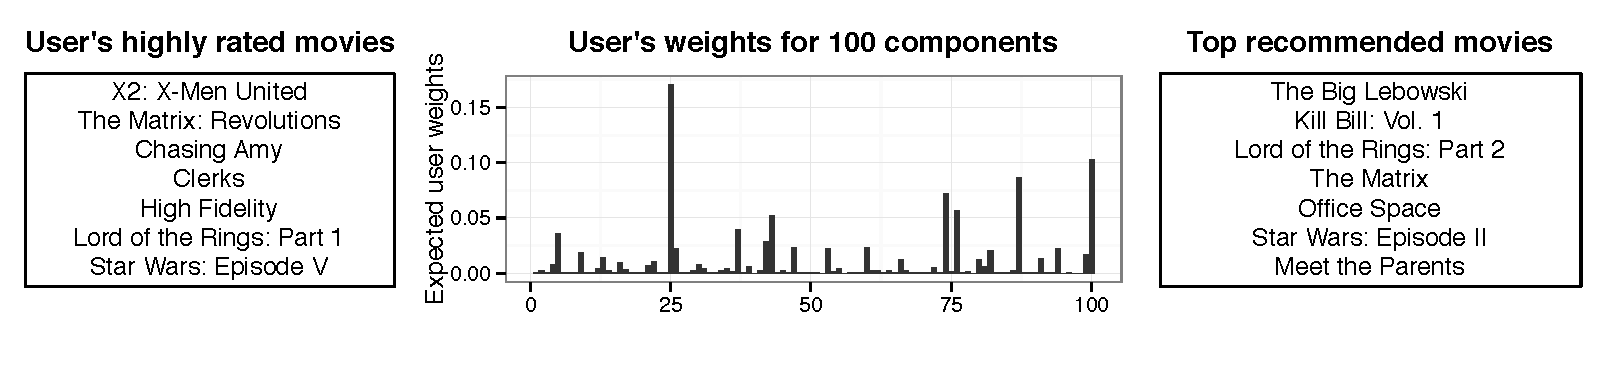
\includegraphics[width=\textwidth]{figures/netflix-exploratory.pdf}\\
\caption{An illustration showing a subset of the highly rated movies
  of a selected user in the Netflix data set~\cite{Koren:2009}, and
  some of the top movies recommended to the user by our algorithm. The
  expected user's $K$-vector of weights $\theta_u$, inferred by our
  algorithm is shown. In our analysis, $K$ was set to 100.}
\label{fig:netflix-illustration}
\end{figure*}


%%
%%\begin{figure}
%%\centering
%%\includegraphics[width=0.8\columnwidth]{figures/movielens-user.pdf}\\
%%\includegraphics[width=0.8\columnwidth]{figures/movielens-item.pdf}\\
%%\caption{The weights of the randomly chosen user $U$ (Top) in the
 %% movielens data set and the weights of her top recommended movie
  %%\emph{Shakespeare in Love} (Bottom) are shown. User $U$ views a
  %%variety of movies, and her weights span a range of factor. User $U$
  %%had 184 views in the data set of movies ranging from Drama, Comedy,
  %%Thriller to Musical. Of these movies, 126 were either 4 or 5
  %%stars. Movies are generally characterized by a sparse set of
  %%factors.}
%%\end{figure}



%% \begin{figure*}[t!]
%% 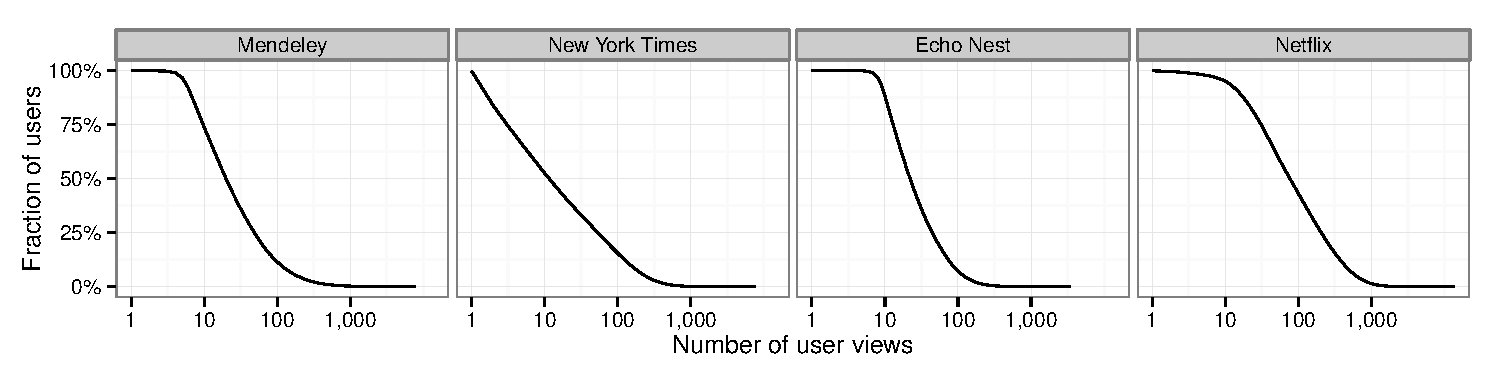
\includegraphics[width=\textwidth]{figures/user_activity_cdf.pdf}
%% \caption{Empirical complimentary cumulative distributions of user
%%   activity on each data set. Each curve shows the fraction of users
%%   who have consumed at least a given number of items. For instance,
%%   slightly less than half of all Netflix users have rated at least
%%   100 movies.}
%% \label{fig:marginals}
%% \end{figure*}


%% \begin{figure*}[t!]
%%   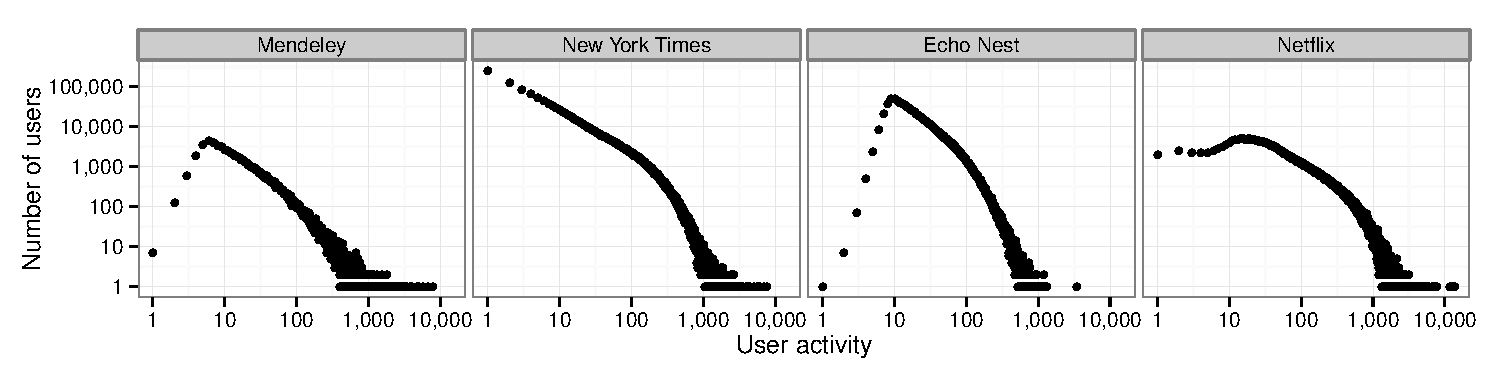
\includegraphics[width=\textwidth]{figures/user_activity.pdf}
%%   \caption{Empirical distributions of user activity on each
%%     dataset. Each plot shows the number of users who have rated a given
%%     number of items. For instance, slightly less than half of all
%%     Netflix users have rated at least 100 movies.}
%% \label{fig:marginals}
%% \end{figure*}

%% \begin{figure*}[t!]
%% 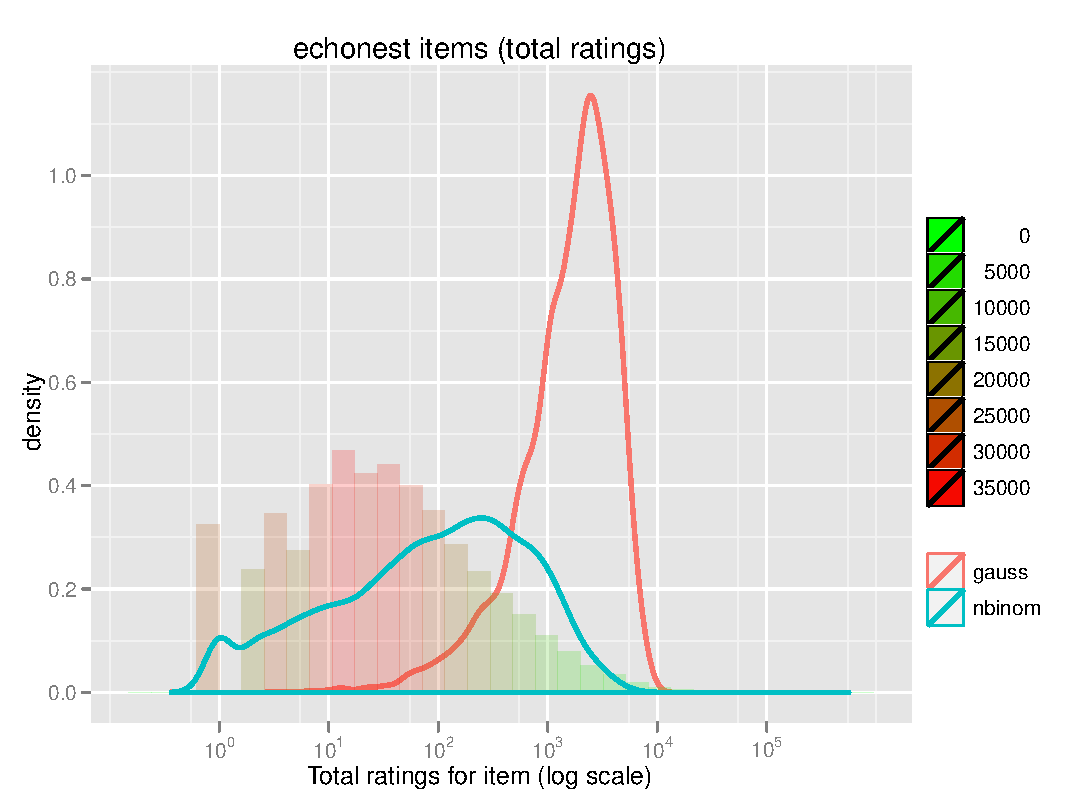
\includegraphics[width=0.33\textwidth]{figures/marginals/echonest.pdf}
%% 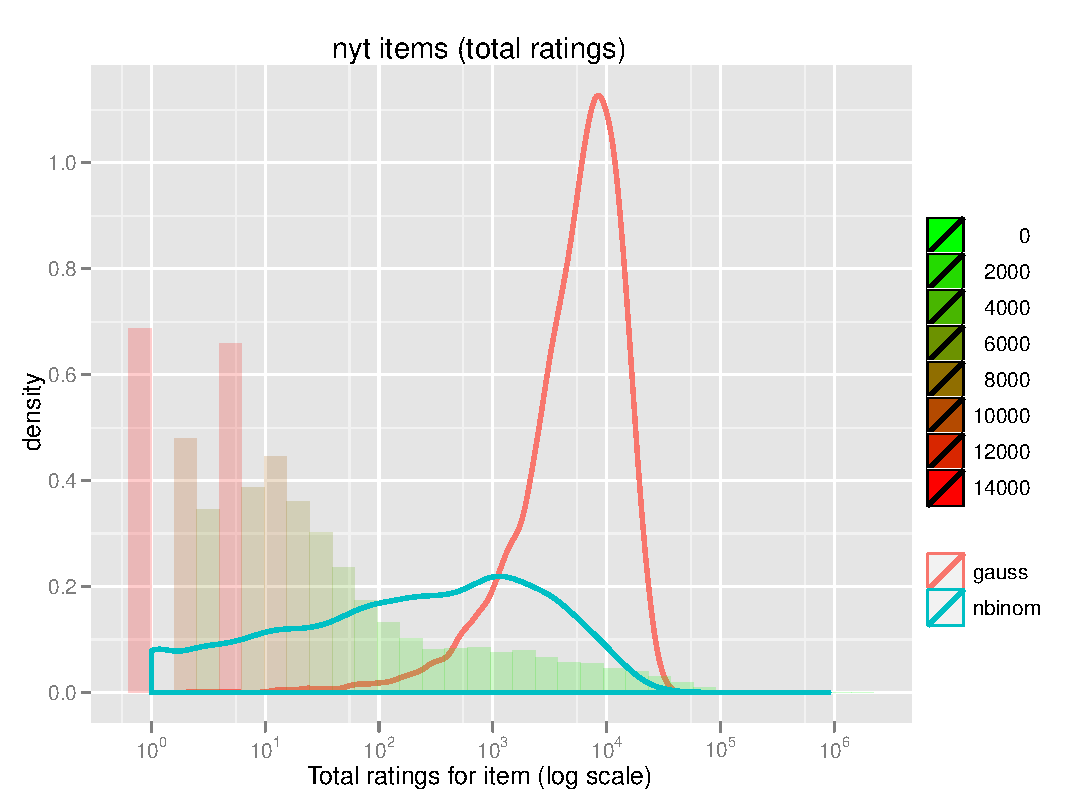
\includegraphics[width=0.33\textwidth]{figures/marginals/nyt.pdf}
%% 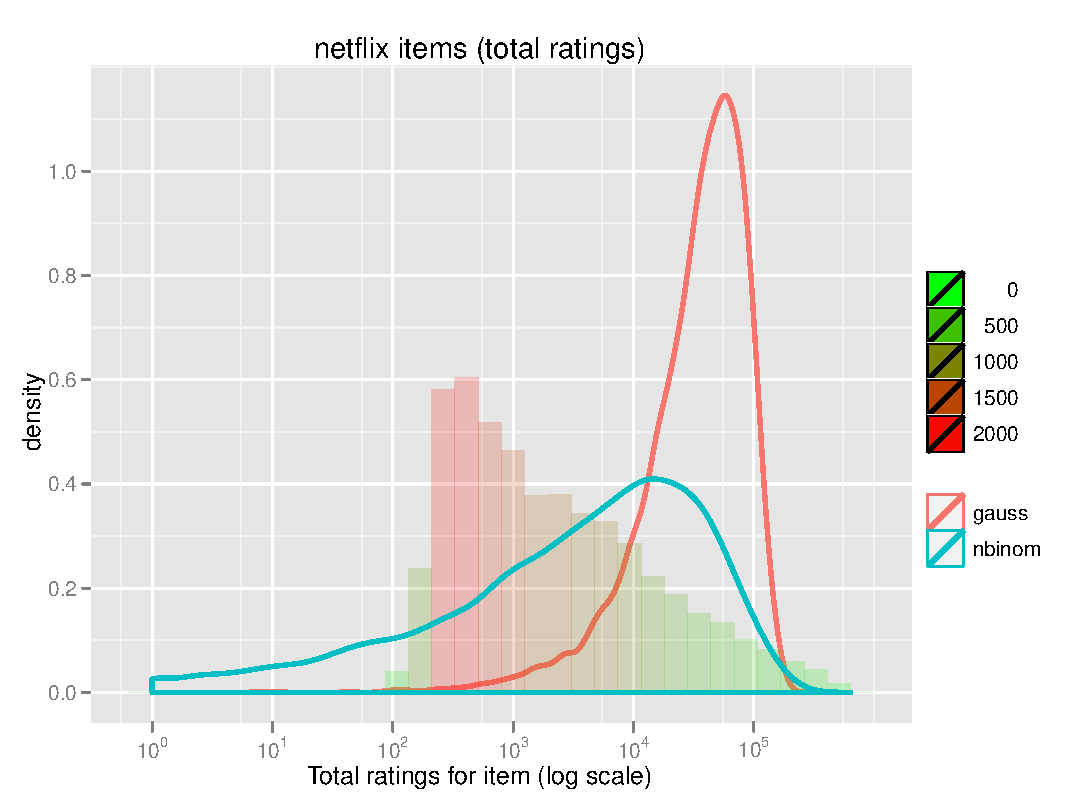
\includegraphics[width=0.33\textwidth]{figures/marginals/netflix.pdf}
%% \caption{Empirical distribution of item popularity on real datasets,
%%   with fitted negative binomial and Gaussian distributions. The
%%   distributions were fit using maximum likelihood estimation. The
%%   negative binomial places significant probability mass on the left
%%   tail, i.e., items with few ratings. The colored bars show that such
%%   items are the most frequent. In contrast, the Gaussian distribution
%%   places negligible mass on the left tail and mainly captures popular
%%   items. The mode of the negative binomial distribution is also closer
%%   to the empirical mode than the Gaussian distribution.}
%% \label{fig:marginals}
%% \end{figure*}

%% Further speed-ups using stochastic variational
%% inference~\cite{Hoffman:2013} let us fit Poisson factorization models
%% to massive data.


\section{Poisson Recommendation}
\label{sec:model}

% !!! review the Gamama and Poisson near the generative process.
% !!! make n_u and n_i the sums
% !!! somewhere we need to make clear how our notation works

We are given data about users and items.  Each user has consumed and
possibly rated a set of items.  The observation $y_{ui}$ is the rating
that user $i$ gave to item $j$, or zero if no rating was given.  (In
simple consumer data, $y_{ui}$ equals one if user $u$ consumed item
$i$ and zero otherwise.)  User behavior data, such as purchases,
ratings, clicks, ``likes'', or ``check ins'', are typically sparse.
Most of the values of the matrix $y$ are zero.

We model this data with factorized Poisson
distributions~\cite{Canny:2004}. Each user $u$ and each item $i$ is
associated with a $K$-vector of positive weights, $\theta_u$ and
$\beta_i$ respectively.  (The number $K$ is fixed in advance.)  The
user/item observation $y_{ui}$ is modeled with a Poisson parameterized
by the inner product of the user's and item's weights $y_{ui} \sim
\poisson(\theta_u^\top \beta_i)$.  This is a variant of probabilistic
matrix factorization~\cite{Salakhutdinov:2008a} but where each user
and item's weights are positive~\cite{Lee:1999} and where the Poisson
likelihood replaces the Gaussian likelihood.

A good collaborative filtering model must capture two basic features
of user and item interactions. First, for any given observation
$y_{ui}$, we expect only a small fraction of the user $u$'s factors
and the item $i$'s factors to be relevant. This favors sparsity in the
weights. Second, there are systematic patterns in the data due to
universally popular items and frequently consuming users. The
literature on recommendation systems suggests that a good model must
capture such heterogeneity across users and items~\cite{Koren2009}. We
therefore extend the Poisson factorization model with a hierarchical
prior structure. We describe our model, and then discuss how it
captures the above properties.

% dmb: jake cites something below
% dmb: also cite "The Dirichlet", old marketing paper

The generative process of the hierarchical Poisson factorization model
(HPF) is as follows:
\begin{enumerate}
\item For each user $u$, choose activity
  \begin{equation*}
    \xi_u \sim \gam(a', a'/b').
  \end{equation*}
\item For each user $u$ and each component $k$, choose weight
  \begin{equation*}
    \theta_{uk} \sim \gam(a, \xi_u).
  \end{equation*}
\item For each item $i$, choose popularity
  \begin{equation*}
    \eta_i \sim \gam(c', c'/d').
  \end{equation*}
\item For each item $i$ and each component $k$, choose weight
  \begin{equation*}
    \beta_{ik} \sim \gam(c, \eta_i).
  \end{equation*}
\item For each user $u$ and item $i$, choose rating
  \begin{equation*}
    y_{ui} \sim \poisson(\theta_u^\top \beta_i).
  \end{equation*}
\end{enumerate}
To enforce sparse weights, the model places a \gam~prior on the
independent weight components. The \gam~distribution
$\gam(x;a,\frac{a}{b})$ parameterized in terms of a shape parameter
$a$ and an inverse scale parameter $\frac{a}{b}$, has a mean of $b$
and a variance of $\frac{b^2}{a}$. For a small shape $a$, most of the
weights will be close to zero, and only a few will be large, resulting
in a sparse representation.

The \gam~rate parameters capture the magnitude of user $u$'s activity
and item $i$'s popularity, respectively.  To capture heterogeneity in
user activity and item popularity, we place a \gam~prior on the rate
parameter $\xi_u$ governing each user $u$ or $\eta_i$ governing each
item $i$. The prior on $\xi_u$ captures the uncertainty around user
$u$'s consumption rate or activity; the prior on $\eta_i$ captures the
uncertainty around item $i$'s popularity among users. Notice that we
fix the shape parameters and share them across users and items.

% dmb: jake cites something below

We also study a sub-class of the HPF where we fix the rate parameters
for all users and items to the same pair of hyperparameters. We call
this model the Bayesian Poisson Factorization (BPF) model.

The HPF model is more powerful than the BPF because it allows for the
sharing of statistical strength. In the HPF, for example, learning
about the number of items consumed by one set of users provides weak,
indirect evidence relevant to other users consumption. This can
improve predictions, especially for users with little activity. A
similar argument favors hierarchy over item popularities. 

Both the HPF and the BPF are conjugate models, resulting in a
computationally efficient inference algorithm.

\subsection{The Posterior distribution}
The posterior distribution of the latent variables $p(\theta, \beta,
\xi, \eta \g y)$ embeds users and items in a latent space of
$K$-dimensional positive vectors. 

We use the HPF to recommend items to users by predicting which of the
unconsumed items each will like.  We rank each user's unconsumed items
by their posterior expected Poisson parameters,
\begin{equation}
  \label{eq:score}
  \textrm{score}_{ui} = \E[\theta_u^\top \beta_i \g y].
\end{equation}
This amounts to asking the model to rank by probability which of the
presently unconsumed items each user will likely consume in the
future.

\subsection{Statistical properties of the HPF model}
With the modeling details in place, we highlight statistical
properties of the model that provide advantages over classical matrix
factorization, and form the basis for scalable inference.

\begin{enumerate}
\item {\bf Modeling the long-tailed distribution of user activity}.
  Figure 3 shows the distributions of user activity on large,
  real-world user/item matrices. These distributions are highly
  skewed, with significant number of users exhibiting much higher
  activity than most users.

Under the BPF and the HPF, the marginal distribution of each user's
ratings, with the item weights held fixed, is a negative binomial.
Let $y_{u} = \sum_{i} y_{ui}$ be the sum of the ratings for user $u$.
Since each of the terms in the sum is a Poisson distribution with rate
$\theta_u^\top \beta_i$, the sum is itself a Poisson random
variable~\cite{Johnson:2005}.
\begin{equation}
  y_u \sim \poisson\left(\theta_u^\top (\textstyle \sum_{i} \beta_{i})\right).
\end{equation}
Holding the item weights fixed, note that the rate of this Poisson is
a sum of scaled Gamma random variables $\beta_{ik} \theta_{uk}$, which
is itself a Gamma variable~\cite{Norman:1994}.  Thus the marginal
distribution of $y_u$ is from an integrated Gamma-Poisson
distribution, which is a negative binomial~\cite{Gelman:1995}.

The negative binomial is a long-tailed distribution that is known to
fit user activity well~\cite{Goodhardt:1984,Dunn1983}.  Figure 3 shows
that the HPF provide good fits to the distribution of user activity on
real-world data.  Classical matrix factorization is based on Gaussian
likelihoods, and the marginal distribution of total user ratings is
also a Gaussian.  The symmetric Gaussian assumption is a poor choice
for modeling long-tailed distributions, and places probability mass on
negative numbers, a setting that never occurs.


\item {\bf Down-weighting the effect of zeros.}
The marginal distribution of $y_u$ is a negative binomial, and this
forces it to down-weight the contribution of the items that each user
did not consume. The reason is that the model has two ways of
explaining that a user does not consume an item: either she is not
interested in it or she would be but has already consumed her allotted
negative-binomial number.  In contrast, a user that consumes an item
must be interested in it.  Thus, the model benefits more from making a
consumed user/item pair more similar than making an unconsumed
user/item pair less similar.

Classical matrix factorization is based on Gaussian likelihoods (i.e.,
squared loss), which gives equal weight to consumed and unconsumed
items.  Consequently, when faced with a sparse matrix and implicit
feedback, i.e., binary consumption data, matrix factorization places
more total emphasis on the unconsumed user/item pairs.  To address
this, researchers have patched the model in complex ways, for example,
by including per-observation confidences~\cite{Koren:2009} or
considering all zeroes to be hidden variables~\cite{Paquet:2013p9197}.
Poisson factorization more naturally solves this problem by better
capturing each user's rate of consumption.

As an example, consider two similar science fiction movies, ``Star
Wars'' and ``The Empire Strikes Back'', and consider a user who has
seen one of them.  The Gaussian model pays an equal penalty for making
the user similar to these items as it does for making the user
different from them---with quadratic loss, seeing ``Star Wars'' is
evidence for liking science fiction, but not seeing ``The Empire
Strikes Back'' is evidence for disliking it.  The Poisson model,
however, will prefer to bring the user's latent weights closer to the
movies' weights because it favors the information from the user
watching ``Star Wars''. Further, because the movies are similar, this
increases the Poisson model's predictive score that a user who watches
``Star Wars'' will also watch ``The Empire Strikes Back''.

\item {\bf Fast inference with sparse matrices.}
The likelihood of the observed data under the BPF and the HPF depends
only on the consumed items, that is, the non-zero elements of the
user/item matrix $y$.  Given the latent variables $\theta_u$ and
$\beta_i$, the Poisson distribution of $y_{ui}$ is
\begin{equation}
  p(y_{ui} \g \theta_u, \beta_i) =
  \left(\theta_u^\top \beta_i\right)^y
  \exp\left\{-\theta_u^\top \beta_i \right\} / y_{ui}!
\end{equation}
Recall the elementary fact that $0! = 1$.  The log probability of the
complete matrix $y$ is
\begin{align}
  \log p(y \g \theta, \beta) =
  & \left(\textstyle \sum_{\{y_{ui} > 0\}}
    y_{ui} \log (\theta_u^\top \beta_i) - \log y_{ui}!
  \right) \\
  & -
  \left(\textstyle\sum_{u} \theta_u\right)^\top \left(\textstyle
    \sum_{i} \beta_i\right).
\end{align}
That this likelihood depends only on the non-zero elements facilitates
inference with sparse matrices.  In contrast, classical matrix
factorization methods, especially when applied to
massive data sets, must address the zeros either through
sub-sampling~\cite{Dror:2012a} or approximation~\cite{Hu:2008p9402}.

\item {\bf }

\end{enumerate}

% dmb: above, maybe add a comment above that this is a heavy-tailed
% realistic distribution for consumer data.  cite goodhardt 1984
% again.


\section{Variational Inference}
\label{sec:inference}

The key computation for the HPF is the posterior distribution of the
user weights $\theta_{uk}$, item weights $\beta_{ik}$, user activity
$\xi_{u}$ and item popularity $\eta_i$ given an observed matrix
of user behavior $y$,
\begin{equation*}
  p(\theta, \beta, \xi, \eta \g y) = \frac{p(\theta | \xi) p(\xi)
    p(\eta) p(\beta | \eta) p(y \g \theta, \beta, \xi, \eta)}
  {\int_{\theta} \int_{\xi} \int_{\eta} \int_{\beta} p(\theta |
    \xi) p(\xi) p(\beta) p(\beta | \eta) p(y \g \theta, \beta, \xi, \eta)}.
\end{equation*}
We need the posterior to form recommendations with the posterior
expectations in \myeq{score}.

As for many Bayesian models of interest, however, the posterior is
intractable to compute exactly.  The problem is with the denominator,
which is the marginal probability of the observed matrix and involves
a complicated and high-dimensional integral.  In this section, we show
how to efficiently approximate the posterior with mean-field
variational inference.

Variational inference is a general strategy for approximating
posterior distributions in complex probabilistic
models~\cite{Jordan:1999,Wainwright:2008}.  Variational inference
algorithms posit a family of distributions over the hidden variables,
indexed by free ``variational'' parameters, and then find the member
of that family that is closest in KL divergence to the true posterior.
(The form of the family is chosen to make this optimization possible.)
Thus, variational inference turns the inference problem into an
optimization problem.  Variational algorithms tend to scale better
than alternative sampling-based approaches, like Monte Carlo Markov
chain sampling, and have been deployed to solve many applied problems
with complex models, including large-scale recommendation~\cite{Paquet:2013p9197}.

We develop mean-field variational inference algorithm for the HPF.  We
first describe the mean-field variational family and the corresponding
variational objective.  We then derive a batch algorithm that fits the
variational distribution by repeatedly cycling through the non-zero
data and updating its estimates of the latent representations. The
simple structure of the algorithm lets us scale our approach to data
with millions of users and hundreds of thousands of items on a single
CPU.

% prem: remove stochastic
%% Finally, we develop a scalable stochastic variational inference
%% algorithm for massive data.  This algorithm repeatedly subsamples
%% users from the matrix and updates its estimates of the latent
%% representations.  

Before beginning these derivations, however, we give an alternative
formulation of the model in which we add a layer of latent variables.
These auxiliary variables allow us to take advantage of some general
results for variational
algorithms~\cite{Ghahramani:2001,Hoffman:2013}.  For each user and
item we add $K$ latent variables $z_{uik} \sim \poisson(\theta_{uk}
\beta_{ik})$, which are integers that sum to the user/item value
$y_{ui}$.  A sum of Poisson random variables is itself a Poisson with
rate equal to the sum of the rates.  Thus, these new latent variables
preserve the marginal distribution of the observation, $y_{ui} \sim
\poisson(\theta_{u}^\top \beta_{i})$.  These variables can be thought
of as the contribution from component $k$ to the total observation
$y_{ui}$.  Note that when $y_{ui} = 0$, these auxiliary variables are
not random---the posterior distribution of $z_{ui}$ will place all its
mass on the zero vector.  Consequently, our inference procedure need
only consider $z_{ui}$ for those user/item pairs where $y_{ui} > 0$.

\subsection{Mean-field variational inference} The latent variables in
the model are user weights $\theta_{uk}$, item weights $\beta_{ik}$,
and user-item contributions $z_{uik}$, which we represent as a
$K$-vector of counts $z_{ui}$.  The mean-field family considers these
variables to be independent and each governed by its own distribution,
\begin{align}
  \label{eq:q}
  q(\beta, \theta, \xi, \eta, z) =& \prod_{i,k} q(\beta_{ik} \g \lambda_{ik})
  \prod_{u,k} q(\theta_{uk} \g \gamma_{uk}) \nonumber\\ 
  & \prod_{u} q(\xi_u \g \kappa_u) \prod_{i} q(\eta_i \g \tau_i)
  \prod_{u,i} q(z_{ui} \g \phi_{ui}).
\end{align}
Though the variables are independent, this is a flexible family of
distributions because each variable is governed by its own free
parameter.  (We postpone specifying the forms of each of these factors
to below.)

After specifying the family, we fit the variational parameters $\nu =
\{\lambda, \gamma, \kappa, \tau, \phi\}$ to minimize the KL divergence to the
posterior
\begin{equation*}
  \nu^* = \arg \min_\nu \textrm{KL}(q(\beta,
  \theta, \kappa, \tau, z \g \nu) || p(\beta, \theta, \kappa, \tau, z \g y)).
\end{equation*}
We then use the corresponding variational distribution $q(\cdot \g
\nu^*)$ as a proxy for the posterior.\footnote{In fact, variational inference
optimizes an equivalent objective that is the KL divergence up to an
additive constant.  But this detail is not needed here.}  The
mean-field factorization facilitates both optimizing the variational
objective and downstream computations with the approximate posterior,
such as the recommendation score of \myeq{score}.

\subsection{Complete conditionals}

Variational inference fits the variational parameters to minimize
their KL divergence to the posterior.  For a large class of models, we
can easily perform this optimization with a coordinate-ascent
algorithm, one in which we iteratively optimize each variational
parameter while holding the others fixed.  Specifically, we appeal to
general results about the class of \textit{conditionally conjugate}
models~\cite{Ghahramani:2001,Hoffman:2013}.  We define the class, show
that the HPF is in the class, and then give the variational inference
algorithm.

A \textit{complete conditional} is the conditional distribution of a
latent variable given the observations and the other latent variables
in the model.  A conditionally conjugate model is one where each
complete conditional is in an exponential family (such as a Gaussian,
Gamma, Poisson, multinomial, or others).  This is a large class of
models.

The HPF, with the $z_{ui}$ variables described above, is a
conditionally conjugate model.  (Without the auxiliary variables, it
is not conditionally conjugate.) For the user weights $\theta_{uk}$,
the complete conditional is a Gamma,
\begin{equation}
  \label{eq:user-weight-cc}
  \theta_{uk} \g \beta, \xi, z, y \sim
  \gam(a + \textstyle \sum_{i} z_{uik}, \xi_u + \sum_{i} \beta_{ik}).
\end{equation}
The complete conditional for item weights $\beta_{ik}$ is symmetric,
\begin{equation}
  \label{eq:item-weight-cc}
  \beta_{ik} \g \theta, \eta, z, y \sim
  \gam(a + \textstyle \sum_{u} z_{uik}, \eta_i + \sum_{i} \theta_{uk}).
\end{equation}
These distributions stem from conjugacy properties between the Gamma
and Poisson. In the user weight distribution, for example, the item
weights $\beta_{ik}$ act as ``exposure'' variables~\cite{Gelman:1995}.
(The roles are reversed in the item weight distribution.) We can
similarly write down the complete conditionals for the user activity
$\xi_u$ and the item popularity $\eta_i$.
\begin{align}
  \label{eq:user-weight-cc}
  \xi_{u} \g \theta \sim
  \gam(a' + \textstyle Ka, b' + \sum_{k} \theta_{uk}).\nonumber\\
  \eta_{i} \g \beta \sim
  \gam(c' + \textstyle Kc, d' + \sum_{k} \beta_{ik}).\nonumber\\
\end{align}

The final latent variables are the auxiliary variables.  Recall that
each $z_{ui}$ is a $K$-vector of Poisson counts that sum to the
observation $y_{ui}$. The complete conditional for this vector is
\begin{equation}
  \label{eq:aux-cc}
  z_{ui} \g \beta, \theta, y \sim \mult\left(y_{ui}, \frac{\theta_{u} 
      \beta_{i}}{\textstyle \sum_{k} \theta_{uk} \beta_{ik}}\right).
\end{equation}
Though these variables are Poisson in the model, their complete
conditional is multinomial.  The reason is that the conditional
distribution of a set of Poisson variables, given their sum, is a
multinomial for which the parameter is their normalized set of rates.
See~\cite{Johnson:2005} (and Appendix A).

\subsection{Variational algorithm}

\begin{figure}
  \begin{framed}
    For all users and items, initialize the user parameters
    $\gamma_u$, $\kappa_u^{\rate}$ and item parameters $\lambda_i$,
    $\tau_i^{\rate}$ to the prior with a small random offset. Set the
    user activity and item popularity shape parameters:
    \begin{align}
      \kappa_u^{\shape} = a + Ka'; \quad \tau_i^{\shape} = c + Kc'\nonumber
    \end{align}

    \vspace{0.1in}

    Repeat until convergence:
    \begin{enumerate}
    \item For each user/item such that $y_{ui} > 0$, update the multinomial:
      \begin{equation*}
        \phi_{ui} \propto \exp\{\Psi(\gamma_{uk}^\shape) - \log
        \gamma_{uk}^{\rate} + \Psi(\lambda_{ik}^\shape) - \log
        \lambda_{ik}^\rate\}.
      \end{equation*}
    \item For each user, update the user weight and activity parameters:
      \begin{align}
        \gamma_{uk}^\shape & = a + \textstyle \sum_{i} y_{ui}
        \phi_{uik} \nonumber\\
        \gamma_{uk}^\rate & = \frac{\kappa_u^{\shape}}{\kappa_u^{\rate}} + \textstyle \sum_i \lambda_{ik}^{\shape} / \lambda_{ik}^{\rate}\nonumber\\
        \kappa_{u}^\rate & = b' + \sum_k \Psi(\gamma_u^{\shape}) - \log(\gamma_u^{\rate})\nonumber
      \end{align}
    \item For each item, update the item weight and popularity parameters:
      \begin{align}
        \lambda_{ik}^\shape & = c + \textstyle \sum_{u} y_{ui}
        \phi_{uik}\nonumber\\
        \lambda_{ik}^\rate & = \frac{\tau_i^{\shape}}{\tau_i^{\rate}} + \textstyle \sum_u
        \gamma_{uk}^{\shape} / \gamma_{uk}^{\rate}\nonumber\\
        \tau_{i}^\rate & = d' + \sum_k \Psi(\lambda_i^{\shape}) -
        \log(\lambda_i^{\rate})\nonumber
      \end{align}
    \end{enumerate}
\end{framed}
\caption{\label{fig:batch}Batch variational inference for Poisson
  factorization.  Each iteration only needs to consider the non-zero
  elements of the user/item matrix.}
\end{figure}

We now derive variational inference for the HPF. First, we set each
factor in the mean-field family (\myeq{q}) to be the same type of
distribution as its complete conditional.  The complete conditionals
for the item weights $\beta_{ik}$ and user weights $\theta_{uk}$ are
Gamma distributions (Equations \ref{eq:user-weight-cc} and
\ref{eq:item-weight-cc}); thus the variational parameters
$\lambda_{ik}$ and $\gamma_{uk}$ are Gamma parameters, each containing
a shape and a rate.  Similarly, the variational user activity
parameters $\kappa_u$ and the variational item popularity parameter
$\tau_i$ are Gamma parameters, each containing a shape and a rate.
The complete conditional of the auxiliary variables $z_{uik}$ is a
multinomial (\myeq{aux-cc}); thus the variational parameter
$\phi_{ui}$ is a multinomial parameter, a point on the $K$-simplex,
and the variational distribution for $z_{ui}$ is $\mult(y_{ui},
\phi_{ui})$.

In coordinate ascent we iteratively optimize each variational
parameter while holding the others fixed.  In conditionally conjugate
models, this amounts to setting each variational parameter equal to
the expected parameter (under $q$) of the complete
conditional.\footnote{It is a little more complex then this.  We must
  be working with the natural parameterization of the corresponding
  exponential families.  For details, see~\cite{Hoffman:2013}.}  The
parameter to each complete conditional is a function of the other
latent variables (by definition) and the mean-field family sets all
the variables to be independent.  These facts guarantee that the
parameter we are optimizing will not appear in the expected parameter.


For the user and item weights, we update the variational shape and
rate parameters.  (We denote shape with the superscript ``shp'' and
rate with the superscript ``rte''.) The updates are
\begin{eqnarray}
  \gamma_{uk} &=& \langle a + \textstyle \sum_{i} y_{ui} \phi_{uik},
  b + \textstyle \sum_i \lambda_{ik}^{\shape} / \lambda_{ik}^{\rate} \rangle \\
  \lambda_{ik} &=& \langle c + \textstyle \sum_{u} y_{ui} \phi_{uik},
  d + \textstyle \sum_u \gamma_{ik}^{\shape} / \gamma_{ik}^{\rate} \rangle.
\end{eqnarray}
These are expectations of the complete conditionals in
Equations~\ref{eq:user-weight-cc} and \ref{eq:item-weight-cc}.  In the
shape parameter, we use that the expected count of the $k$th item in
the multinomial is $\E_q[z_{uik}] = y_{ui} \phi_{uik}$. In the rate
parameter, we use that the expectation of a Gamma variable is the
shape divided by the rate.

For the variational multinomial the update is
\begin{equation}
  \phi_{ui} \propto \exp\{\Psi(\gamma_{uk}^\shape) - \log
  \gamma_{uk}^{\rate} + \Psi(\lambda_{ik}^\shape) - \log
  \lambda_{ik}^\rate\},
\end{equation}
where $\Psi(\cdot)$ is the digamma function (the first derivative of
the log $\Gamma$ function).  This update comes from the expectation of
the log of a Gamma variable, for example $\E_q[\log \theta_{uk}] =
\Psi(\gamma_{nk}^\shape) - \log \gamma_{nk}^{\rate}$.

The coordinate ascent algorithm iteratively executes these updates
(see \myfig{batch}).  This algorithm is very efficient on sparse
matrices. In step 1, the algorithm only needs to update variational
multinomials for the non-zero user/item observations $y_{ui}$.  In
steps 2 and 3, the sums over users and items also only need to
consider non-zero observations.  In contrast, fitting a traditional
matrix factorization with squared loss must iteratively consider every
cell of the matrix, both zeros and non-zeros. This makes matrix
factorization difficult to fit with large matrices, though there are
innovative solutions based on stochastic
optimization~\cite{Mairal:2010}.

%% Implemented in parallel, the coordinate updates are equal to the
%% natural gradient of the variational objective. We found that following
%% these natural gradients~\cite{Hoffman:2013, Honkela:2008,Sato:2012}
%% (with step size one) resulted in a better way to fit the objective.
%% The algorithm in \myfig{batch} remains the same, except we now compute
%% steps 2 and 3 in parallel, updating the variational shape and rate
%% parameters of all users and items using the multinomial $\phi_{ui}$
%% parameters.


\begin{figure*}[t!]
\centering
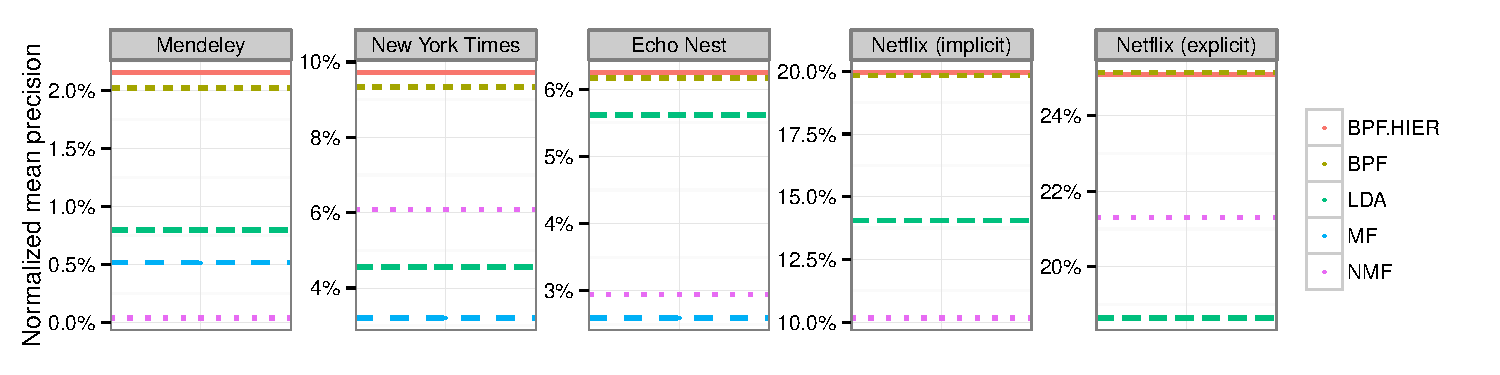
\includegraphics[width=\textwidth]{figures/mean_precision_at_10.pdf}\\
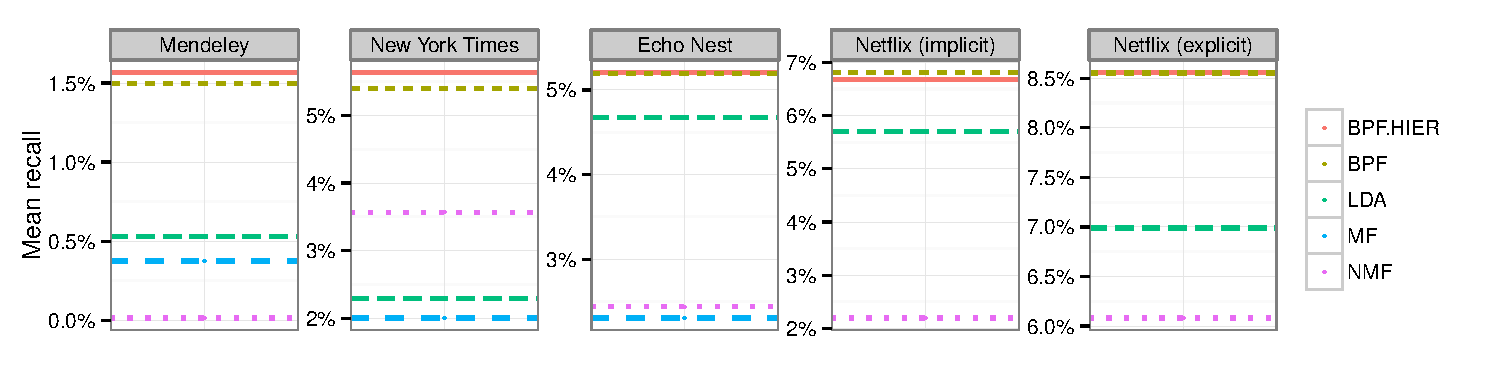
\includegraphics[width=\textwidth]{figures/mean_recall_at_10.pdf}\\
\caption{Predictive performance on datasets. The top and bottom plots
  show normalized mean precision and mean recall at 10
  recommendations, respectively.}
\label{fig:precision_recall_at_10}
\end{figure*}


%% \begin{figure*}[t!]
%% \centering
%% 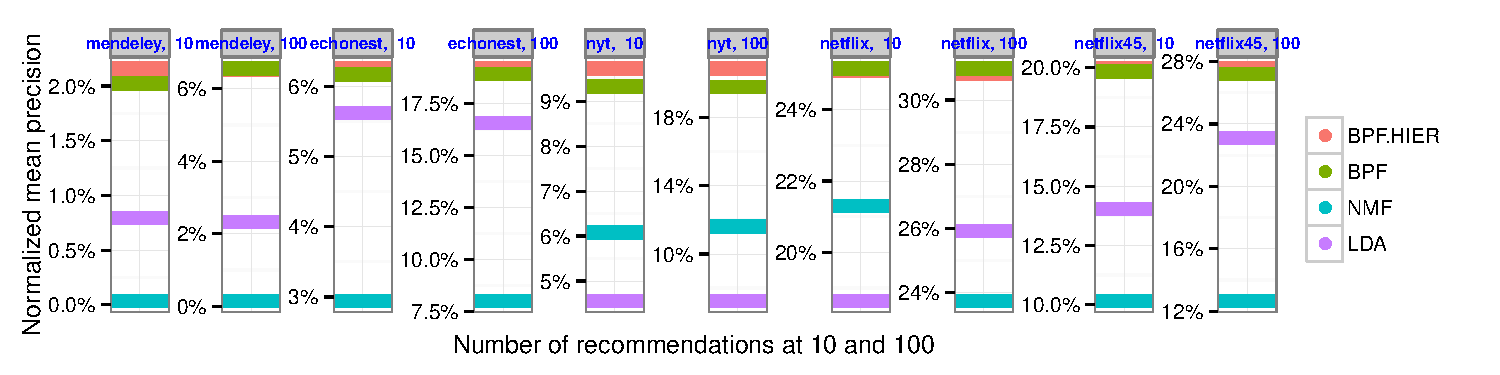
\includegraphics[width=\textwidth]{./figures/meanprecision2.pdf}\\               
%% 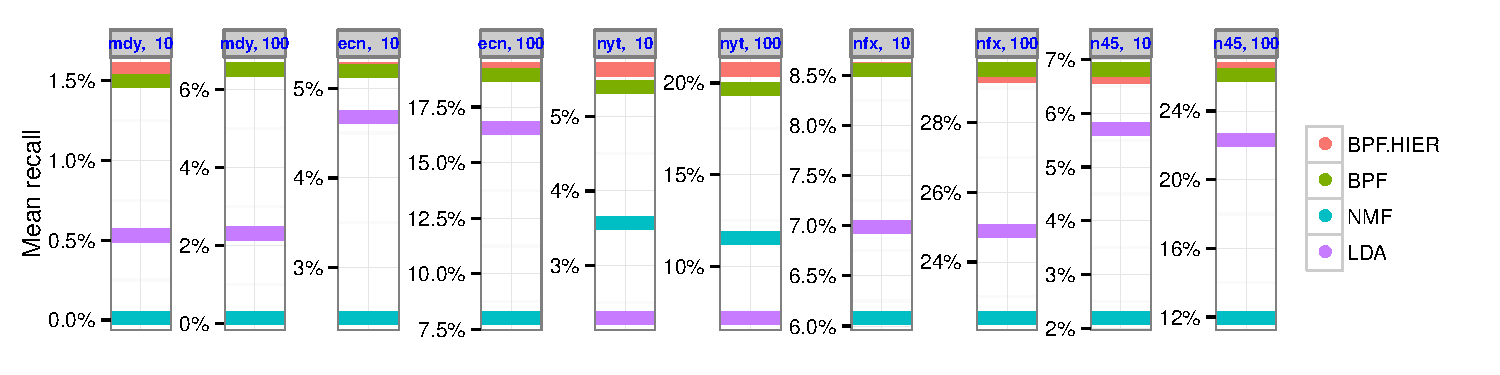
\includegraphics[width=\textwidth]{./figures/meanrecall2.pdf}\\               
%% 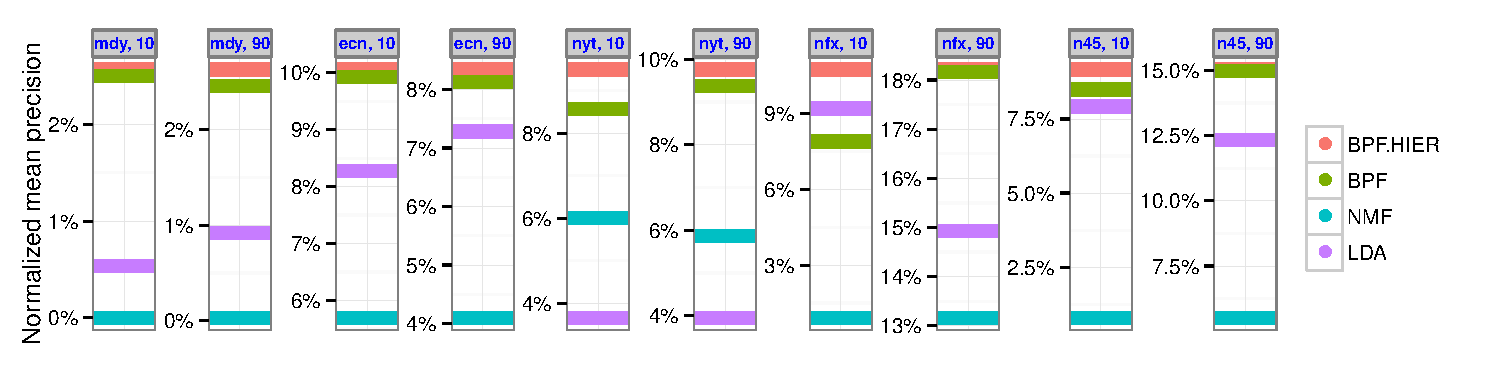
\includegraphics[width=\textwidth]{./figures/useractivity-meanprecision2.pdf}\\
%% 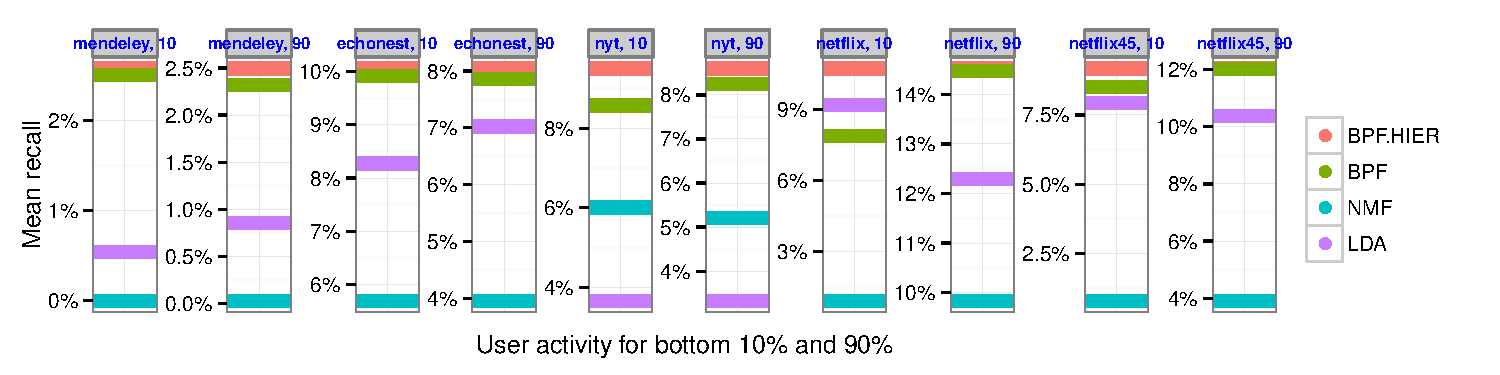
\includegraphics[width=\textwidth]{./figures/useractivity-meanrecall2.pdf}\\
%% \caption{Predictive performance on datasets. The top two plots show
%%   normalized mean precision and mean recall at 10 and 100
%%   recommendations. The bottom two plots show normalized mean precision
%%   and mean recall for the bottom 10\% and bottom 90\% of users by
%%   activity.}
%% \label{fig:precision_by_M}
%% \end{figure*}


\section{Empirical Study}
We studied the Bayesian Poisson Factorization (BPF) algorithm of
Figure~\ref{fig:batch} on a variety of large real data sets. We
demonstrate in this section that BPF definitively outperforms matrix
factorization (MF) in predictive performance on all data sets.
\begin{figure*}[th]
\centering
\subfigure[]{
  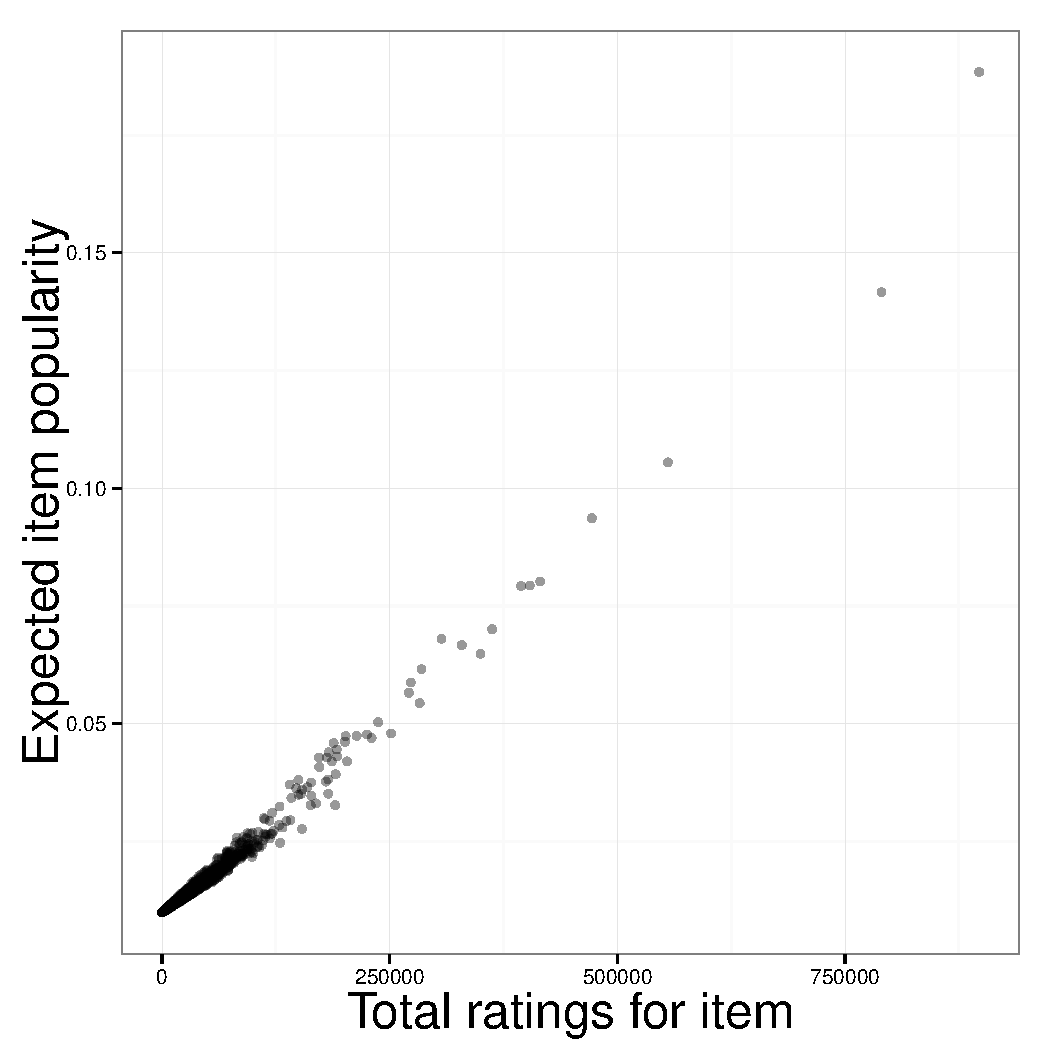
\includegraphics[width=0.45\textwidth]{./figures/nyt/itemsrate.pdf}
}
\subfigure[]{
  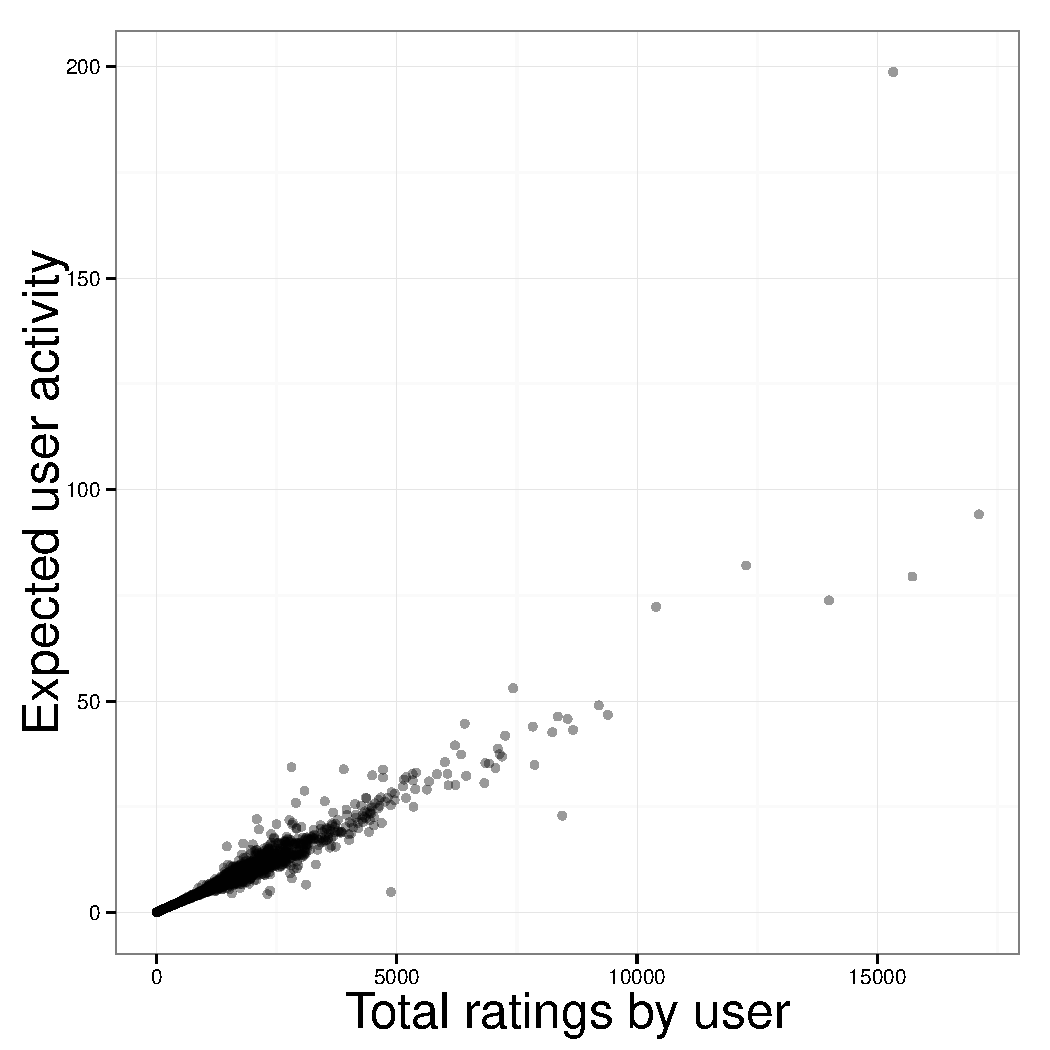
\includegraphics[width=0.45\textwidth]{./figures/nyt/userrate.pdf}
}
\caption{Popularity of articles on the NYT dataset.}
\label{fig:nyt-expl}
\end{figure*}


\begin{table*}
\centering
\caption{Most popular articles in the NYT dataset}
\begin{tabular}{|l|r|r|} \hline
Title & Expected popularity & Number of factors\\\hline
Blasts at Boston Marathon Kill 3 and Injure 100 & 0.043 & 1\\\hline
FBI Posts Images of Pair Suspected in Boston Attack & 0.042 & 1\\\hline
Bombing Inquiry Turns to Motive and Russia Trip & 0.037 & 1\\\hline
War Zone at Mile 26: 'So Many People Without Legs' & 0.025 & 1\\\hline
Suspects Seemed Set for Attacks Beyond Boston & 0.031 & 1\\\hline
In Signal Image From Boston Bombing a Father Sees His Son & 0.029 & 1\\\hline
Skeleton in British Parking Lot Hailed as Richard III & 0.027 & 4\\\hline
Surviving Suspect is Charged by US in Boston Attack & 0.027 & 1\\\hline
The Boy With A Thorn In His Joints & 0.026 & 3\\\hline
Drowned in a Stream of Prescriptions & 0.025 & 3\\\hline
\end{tabular} 
\end{table*}

{\bf Data Sets.} We study the Bayesian Poisson Factorization algorithm
in Figure~\ref{fig:batch} on several large data sets:
\begin{itemize}
\item The {\bf New York Times} data set with 1,615,675 users, 103390
  articles movies and 80,071,435 ratings.
\item The {\bf Netflix} data set~\cite{Koren:2009} with 480,000 users,
  17,770 movies and 100 million ratings is similar to MovieLens but
  significantly larger. Unlike the MovieLens data, the Netflix data
  set is highly skewed and is more realistic: Some users rate more
  than 10,000 movies, while others rate less than
  5~\cite{Salakhutdinov:2008a}.
\item The {\bf Mendeley} data set~\cite{Jack:2010} of scientific
  articles is a binary matrix of
  80,000 users and 260,000 articles, where an article is considered
  consumed by a user if it's in the user's library.
\item The {\bf Echo Nest} music data set~\cite{Bertin-Mahieux:2011} consists of 1
  million users, 385,000 distinct songs and 48 million (user, song,
  play count) triplets.
\end{itemize}

The scale and diversity of these data sets enables a robust evaluation
of our algorithm. Both the Mendeley and the Echo Nest data sets are
sparse in comparison to the movie data: only 0.001\% of the matrix of
ratings is non-zero in Mendeley, while 1\% of the ratings are non-zero
in Netflix and 4\% in MovieLens. Further, the Mendeley data set has
many more articles than users.


%% users watching movies on MovieLens~\cite{Koren:2009} and
%% Netflix~\cite{Herlocker:1999}, individuals listening to songs in the
%% Echo Nest data set~\cite{Bertin-Mahieux:2011}, and academics reading
%% scientific articles via Mendeley~\cite{Jack:2010}.


%% The MovieLens data set consists of 1 million ratings
%% from 6040 users on 4000 movies. Each movie is associated with a title
%% and a category. The Netflix data set is similar to---but significantly
%% larger than---the MovieLens data set, consisting of 100M ratings from
%% 480,000 users on 17770 movies.

{\bf Pre-processing and training.} We now describe how we the
pre-process the input data, train the model, and assess the predictive
accuracy on a held-out set.

Prior to training, we randomly select 20\% of ratings in each data set
to be used as a held-out test set comprised of items that the user
has consumed. During training, these test set observations are treated
as zeros. Additionally, we set aside 1\% of the training ratings as a
validation set and use it to determine the convergence of our
algorithm.

During training, the input to our algorithm is the count data, for
example, the movie ratings or the play count of a song. Notice that
for the Mendeley data set, the input is binary. During training, we
fix the shape and rate hyperparameters. This gives good performance on
our validation set. We find that the algorithm is insensitive to small
changes in the hyper-parameters.

%% corresponding to ratings or the play count of a song. Optionally, the
%% algorithm can transform the input count data to binary before training
%% the model.  For example, the observation $y_{ui}$ is set to one only
%% if the $u$-th user explicitly rated the $i$-th movie. (We denote the
%% algorithm that fits the transformed data, BPF-binary or BPF-BIN.)

We terminate the training process when the BPF algorithm
converges. The convergence is measured by computing the prediction
accuracy on our validation set. We approximate the probability that a
user consumed an item using the variational approximations to
posterior expectations of $\theta_u$ and $\beta_i$, and compute the
average predictive log likelihood of the validation ratings. The BPF
algorithm stops when the change in log likelihood is less than
0.0001\%.

\begin{figure*}[t!]
\centering
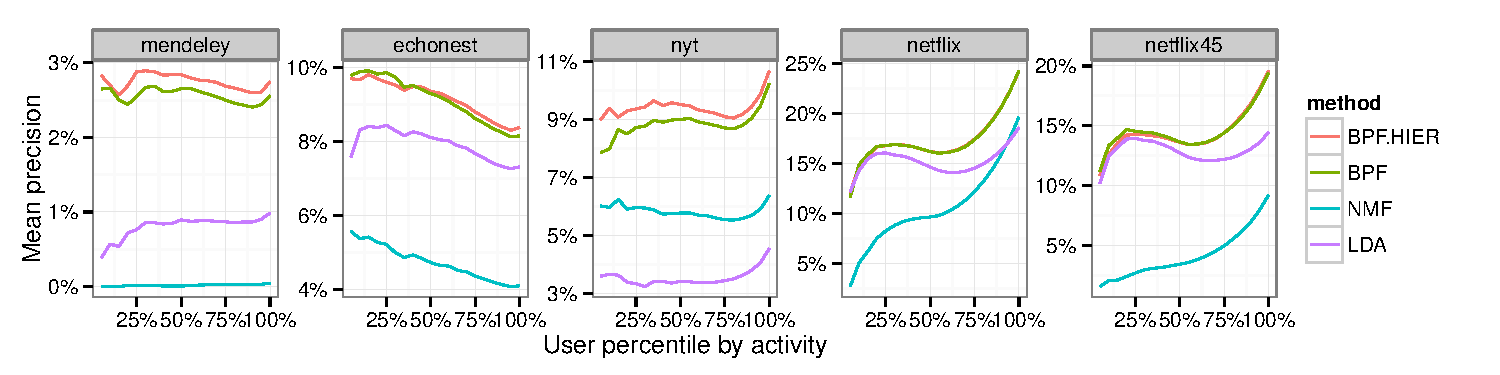
\includegraphics[width=\textwidth]{figures/mean_precision_by_user_percentile.pdf}\\
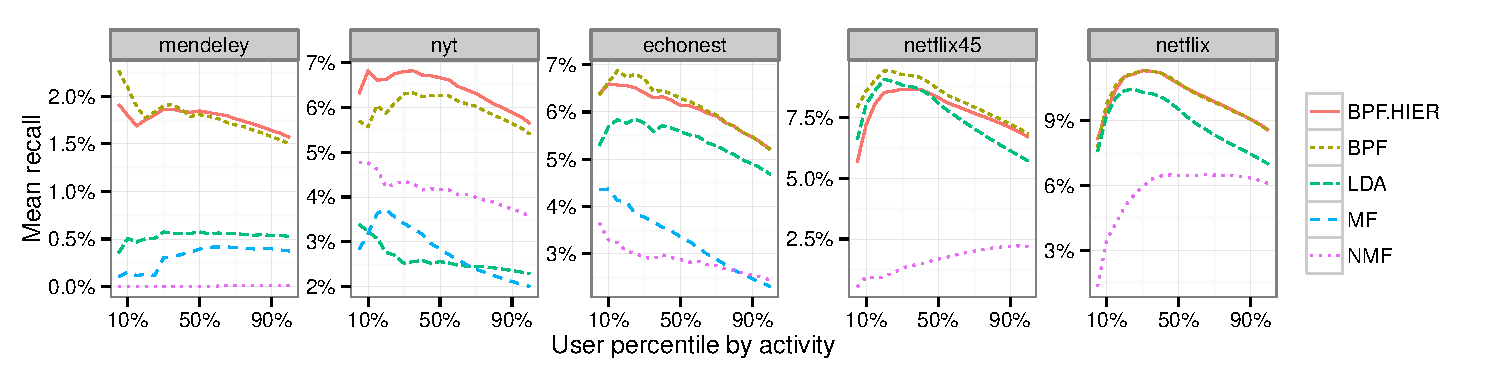
\includegraphics[width=\textwidth]{figures/mean_recall_by_user_percentile.pdf}\\
\caption{Predictive performance across users. The top and bottom plots
  show normalized mean precision and mean recall at 10
  recommendations, respectively, by user activity.}
\label{fig:precision_recall_by_user_activity}
\end{figure*}


{\bf Exploratory analysis.} The fitted model can be explored to
discover latent structure among items and users and to confirm that
the model is capturing the components in the data in a reasonable
way. For example, in \myfig{components} we illustrate the components
discovered by our algorithm on the MovieLens and the Netflix movie
ratings and the Mendeley data of users and scientific articles. For
each data set, the illustration shows the top 10 items---items sorted
in decreasing order of their expected weight $\beta_i$---from three of
the 100 components discovered by our algorithm. These components
naturally organize the movies and articles, and enable recommendation
of new items to the user.

In \myfig{movielens-illustration} we show a subset of the highly rated
movies of a user from the MovieLens data
set~\cite{Herlocker:1999}. The top 15 movies recommended to this user
using the trained BPF model, are also shown. The user's ratings are
for primarily drama movies. We movies BPF recommends closely resemble
the types of drama movies she is interested in, for example,
``Children's drama'' or ``War drama''. The expected user's $K$-vector
of weights $\theta_u$, inferred by our algorithm, is shown in
\myfig{movielens-illustration}. In our analysis, $K$ was set to
100. The $\theta_u$ are not sparse because the user's views span a
range of movies in the small data set.

{\bf Testing.} During testing, we generate the top $M$ recommendations
for each user as those items with the highest predictive score in
\myeq{score}. The ranked list of items predicted for each user
includes items in the test set, as well as items in the training set
that were zeros. We compute precision-at-$M$, which measures the
fraction of the top $M$ recommendations present in the test set,
varying $M$ from 10 to 100 items. Likewise, we compute recall-at-$M$,
which captures the fraction of items in the test set present in the
top $M$ recommendations.

%% In contrast, the Echo Nest and Mendeley data sets contain implicit
%% feedback on which songs and scientific papers users have consumed.

%% !!! prem: assume BPF-binary for now. will try to move to BPF-bias
%% where the non-binary observations are fit

{\bf Baselines.} We compare our performance against traditional matrix
factorization (MF). Ratings are modeled as
\begin{equation*}
  y_{ui} = c + a_u + b_i + \theta_u^\top \beta_i,
\end{equation*}
where $c$ denotes a global intercept term, $a_u$ captures the relative
activity of the $u$-th user, and $b_i$ accounts for the popularity of
the $i$-th item. The final term quantifies interactions between a user
and item via their K-dimensional latent factors, with $\theta_u$ specifying
the user's interests and $\beta_i$ describing the item's attributes. The
model is fit by stochastic gradient descent using the open source
Vowpal Wabbit package~\cite{Weinberger:2009} to minimize squared error
between predicted and actual ratings.

We note that while BPF takes only the non-zero observed ratings as
input, traditional matrix factorization requires that we provide
explicit zeros in the ratings matrix as negative examples. In
practice, this amounts to either treating all missing ratings as zeros
and down-weighting to balance the relative importance of observed and
missing ratings~\cite{Hu:2008p9402}, or generating negatives by
randomly sampling from missing ratings in the training
set~\cite{Dror:2012a}.  We take the latter approach for computational
convenience, employing two popular sampling schemes. In the first,
denoted MF-UNI, we sample a fixed number of negative examples
uniformly at random for each user such that there are approximately
the same number of positive and negative examples. In the second,
termed MF-POP, we sample users by activity---the number of items rated
in the training set---and items by popularity---the number of training
ratings an item received. 

For MF, we cross-validate over the gradient update step size, the
strength of an $L_2$-regularization term across all weights, and the
number of passes over the training data. This results in a reasonably
expensive grid search, from which we select
the model that performs best on the validation set for each data set.

%% \begin{figure*}[t]
%% \centering
%% \includegraphics[width=\textwidth]{./figures/precision_by_user_activity_and_method.pdf}\\
%% \label{fig:precision_by_user_activity}
%% \caption{Precision at 100 recommendations by user activity across data sets and methods.}
%% \end{figure*}

%% \begin{figure*}
%% \centering
%% 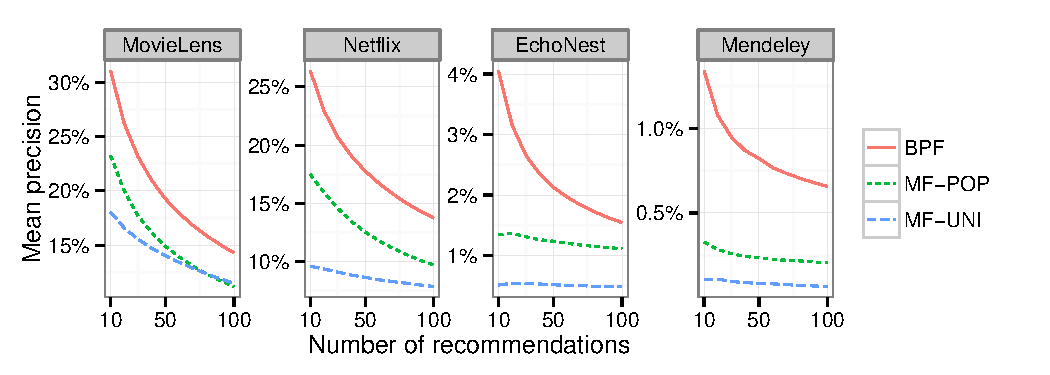
\includegraphics[width=\textwidth]{../output/figures/echonest_and_mendeley/mean_precision_by_method.pdf}\\
%% \includegraphics[width=\textwidth]{../output/figures/echonest_and_mendeley/precision_by_user_activity_and_method.pdf}\\
%% \includegraphics[width=\textwidth]{../output/figures/echonest_and_mendeley/mean_coverage_by_method.pdf}\\
%% \end{figure*}

%% {\bf Results and analysis.} \myfig{precision_by_M} shows the mean
%% precision of the BPF and the MF algorithm as we vary $M$, the number
%% of recommendations. As shown in \myfig{precision_by_M}, BPF
%% outperforms MF on all data sets by a sizeable margin---as much as 8
%% percentage points. Likewise, BPF shows similar gains in recall over
%% traditional MF approaches, indicated in \myfig{recall_by_M}. A
%% relatively high fraction of items recommended by BPF are found to be
%% relevant, and many relevant items are recommended.

%% We also study precision as a function of user activity to investigate
%% for which kinds of users the algorithm performs
%% well. \myfig{precision_by_user_activity} highlights the results in
%% further detail, showing the precision at 100 recommendations for users
%% of varying activity. BPF provides increasingly better performance for
%% more active users.  On the Mendeley data set, BPF performs better for
%% users with less than 1000 articles (BPF does better over all.)  On all
%% other data sets, BPF performs better than MF with all types of users.

%% In all results, MF-POP outperforms MF-UNI, which is indicative of
%% problems with the squared loss objective approximated by MF-UNI.

%% As expected, we see that BPF provides
%% increasingly better recommendations for more active users, and that
%% BPF outperforms MF on the Netflix, MovieLens, and Echo Nest data sets
%% by this measure as well as mean precision across all users.

%% On the Mendeley data set, BPF performs better for users with less than
%% 1000 articles in their library, but MF has better precision than BPF for
%% the small set of users with more than 1000 papers in their library. 

%% !!! prem: need to confirm by looking at actual values; investigate
%\newpage

\begin{figure*}
\centering
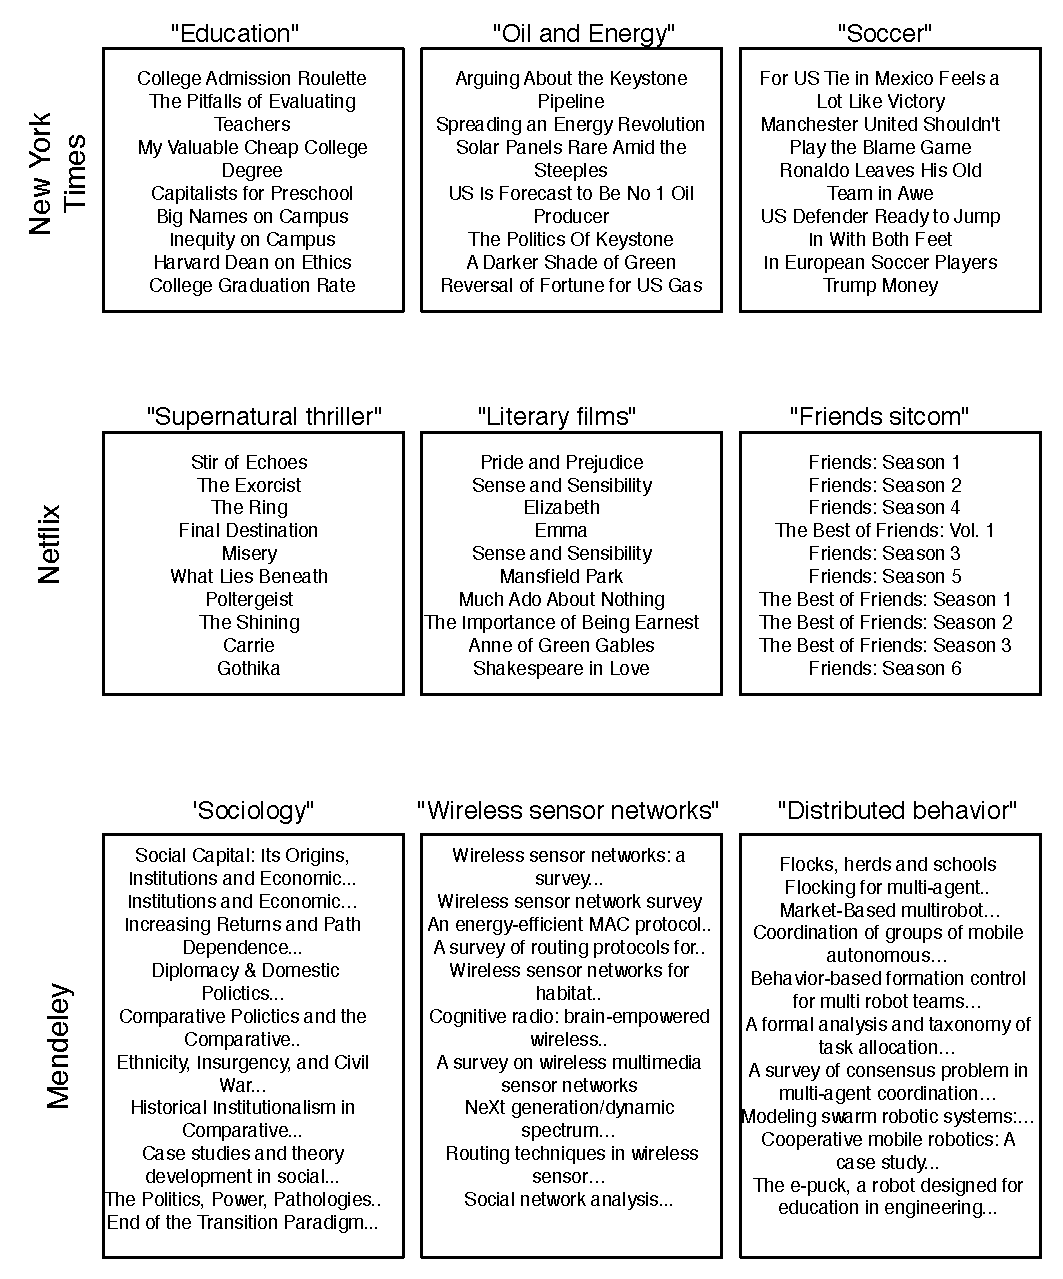
\includegraphics[width=\textwidth]{./figures/components.pdf}
\caption{The top 10 items by the expected weight $\beta_i$ from three
  of the 100 components discovered by our algorithm.}
\label{fig:components}
\end{figure*}

\section{Related work}
The roots of Poisson factorization come from nonnegative matrix
factorization~\cite{Lee:1999}, where the objective function is
equivalent to a factorized Poisson likelihood.  The original NMF
update equations have been shown to be an expectation-maximisation
(EM) algorithm for maximum likelihood estimation of a Poisson model
via data augmentation~\cite{Cemgil:2009}.

Placing a Gamma prior on the user weights gives the GaP
model~\cite{Canny:2004}, which was developed as an alternative text
model to latent Dirichlet allocation (LDA)~\cite{Blei:2003b}. Placing
a Gamma prior on both the user and item weights gives the
Probabilistic Factor Model (PFM)~\cite{Ma:2011}.

A difference between our treatment and GaP is that GaP fits the item
weights with maximum likelihood via the expectation maximization
algorithm. We approximate the full posterior with variational
inference. Further, our model places a hierarchical prior structure
using Gamma priors on weights, and Gamma priors on user and item rate
parameters.  Placing priors on both sets of weights further
regularizes the model and lets us use the same inferential machinery
in both user-space and item-space. 

We note that GaP was developed as an alternative to LDA. In Appendix
A, we show that LDA can be reinterpreted as an instance of Poisson
factorization where we condition on the user counts and use an
alternative prior on the item weights. This relationship has also been
explored in ~\cite{Inouye:2014}.

Although the PFM~\cite{Ma:2011} model is the same as the BPF, the PFM
was aimed at a particular application---that of recommending
web-sites---while we demonstrate improved performance on a variety of
recommendation tasks. Further, we study why Poisson factorization
based models outperform others in recommendation. We also extended the
BPF with a hierarchical prior structure to capture the skew in user
activity and item popularity. Capturing these biases is important for
predictive performance~\cite{Koren:2009}. Again, we approximate the
full posterior with variational inference, while PFM uses Maximum a
posteriori estimation

% prem: removed reference to stochastic inference
%       we should add this in future work/discussion
%% Furthermore, using variational inference opens the door to scaling to
%% massive data sets, even larger than the data sets we analyze in this
%% paper, using stochastic variational inference~\cite{Hoffman:2013} (see
%% \mysec{inference}).

Independently of GaP, Bayesian Poisson factorization has been studied
in the signal processing community for performing source separation
from spectrogram data~\cite{Cemgil:2009,Hoffman:2012}.  This research
includes variational approximations to the posterior, though the
issues and details around spectrogram data differ significantly from
user behavior data we consider and our derivation below (based on
auxiliary variables) is more direct.  As future work, the methods
developed here could lead to improved methods for massive simultaneous
analysis of audio spectrograms. 

In the context of network data, a Poisson model of overlapping
communities was described by the authors of ~\cite{Ball:2011}, and has
been shown to work well in recovering overlapping communities in
network data~\cite{Gopalan:2013}.  As with GaP, this model is
unregularized and the authors fit the model with maximum likelihood
via expectation maximization.

There has been significant research on Bayesian nonparametric Poisson
factor models. Using a Beta-Negative-Binomial process prior for
Poisson factor analysis the authors of ~\cite{Zhou:2012} demonstrate
that NMF, LDA and GaP are special cases of a finite approximation of
their model. Both BPF and HPF does not immediately fall out of their
framework, and placing Bayesian nonparametric priors on our models is
an ongoing research effort.

We discuss further differences between our method and previous work on
matrix factorization in the empirical results below.

% !!! add reference to canny's click data
% !!! add reference to SIGIR
XXX \cite{Marlin:2009,Marlin:2012,Elkan:2008,Ma:2011}

\section{Discussion}
We have demonstrated that Poisson factorization is an efficient and
effective means of generating high quality recommendations across a
variety of data sets ranging from movie views to scientific article
libraries. It significantly outperforms a number of leading methods in
modeling implicit behavior data without the need for ad hoc
modifications. Variational inference for HPF scales to massive data
and differs from traditional methods in its ability to capture the
heterogeneity amongst users and items, accounting for the wide range
of activity and popularity amongst them, respectively. The HPF
algorithm is a robust, off-the-shelf tool, providing high accuracy
even with fixed hyperparameter settings.

%%% recsys-prem !!! added note about SVI here (removed from intro)

Finally, we emphasize that HPF is more than just one method---it is
the simplest in a class of probabilistic models with these properties,
and has already been extended to a combined model of article content
and reader ratings~\cite{gopalan2014content}, and a Bayesian
nonparametric model that adapts the dimensionality of the latent
representations~\cite{gopalan2014bayesian}.

A notable innovation in Gaussian MF is the algorithm
of~\cite{Hu:2008p9402} that explicitly downweights zeros using
confidence parameters. We presented the empirical study in this paper
comparing to the Gaussian MF with subsampled
zeros~\cite{Koren:2009}. Our ongoing work includes bringing the
confidence-weighting of~\cite{Hu:2008p9402} into HPF.
%% To provide a fair
%% comparison to the algorithm of ~\cite{Hu:2008p9402} we need to bring
%% the confidence-weighting of~\cite{Hu:2008p9402} into HPF. 
This will allow downweighting of the zeros beyond that provided
implicitly by Poisson factorization. Our initial experiments show that
even without the downweighting, HPF provides better predictive
performance (measured using the mean rank of recommended items) for
all but the ``heaviest'' portion of the long tail of items, consisting
of the least popular items in the data sets.

%% we present our empirical study
%% without hu et al., but discuss the need to downweight the zeros on
%% even heavier tailed data sets.  we can note that PF dominates gaussian
%% factorization everywhere, but one innovation in gaussian factorization
%% is hu et al. (even if it is unprincipled).  we can talk about ``pilot
%% studies'' against hu et al. which found better performance in most
%% cases, and always for the more popular items.  an area of future work
%% to bring its intuition into PF.

%% This will allow us to provide a fair comparison to the Gaussian
%% MF with downweighted zeros~\cite{Hu:2008p9402}. 

%% , we are comparing to the Gaussian
%% MF with downweighted zeros~\cite{Hu:2008p9402}.

%%  included the 

%% Future work 

%% exploring modifications to BPF to incorporate
%% additional features---e.g., user and item metadata---as well as
%% stochastic inference to scale to massive data sets and Bayesian
%% non-parametric extensions~\cite{Zhou:2012}.


%% In settings where there are many more items than the typical user
%% can consume, unobserved consumption is likely explained by finite
%% attention, as opposed to an active dislike for the associated
%% content. Likewise, a user's choice in selecting a particular set of
%% items amongst the many available options is a relatively strong
%% indicator of her interests. BPF captures these features of sparse user
%% data via the Poisson likelihood, which appropriately balances strong
%% signals of consumption with weaker signals of unobserved activity.

%% Conveniently, the same Poisson likelihood also leads to
%% computationally efficient inference on sparse data sets, as it requires
%% evaluation of only the consumed user-item pairs, which comprise a
%% small fraction of all possible observations. This avoids the issue
%% faced by traditional matrix factorization in down-weighting or sampling
%% negative examples during training. In addition to this computational
%% advantage, BPF empirically outperforms classical MF across a wide array
%% of data sets---from movies to music to scientific articles---in
%% recommending relevant content to users.

%Future work includes exploring modifications to BPF to incorporate
%additional features---e.g., user and item metadata---as well as
%stochastic inference to scale to massive data sets.



%% There has also been significant research on Bayesian nonparametric
%% Poisson factor models. Using a Beta-Negative-Binomial process prior
%% for Poisson factor analysis the authors of ~\cite{Zhou:2012}
%% demonstrate that NMF, LDA and GaP are special cases of a finite
%% approximation to their model. Inference for the models
%% in~\cite{Zhou:2012} do not scale to the size of datasets we consider
%% here.


\small{
  \bibliographystyle{abbrv}
  \bibliography{bib}
}

\newpage
\appendix
\section{Appendix A: The variational algorithm}
Given an observed matrix of user behavior $y$, we would like to
compute the posterior distribution of user preferences $\theta_{uk}$,
item attributes $\beta_{ik}$, user activity $\xi_u$ and item
popularity $\eta_i$, $p(\theta, \beta, \xi, \eta \g y)$.  Our
derivation of the variational algorithm for HPF makes use of
general results about the class of \textit{conditionally conjugate}
models~\cite{Ghahramani:2001,Hoffman:2013}.  We define the class, show
that HPF is in the class, and then derive the variational
inference algorithm.

{\bf Complete conditionals.}  Variational inference fits the
variational parameters to minimize their KL divergence to the
posterior. For the large class of conditionally conjugate models, we
can easily perform this optimization with a coordinate-ascent
algorithm, one in which we iteratively optimize each variational
parameter while holding the others fixed.  A \textit{complete
conditional} is the conditional distribution of a latent variable
given the observations and the other latent variables in the model.  A
conditionally conjugate model is one where each complete conditional
is in an exponential family.

HPF, with the $z_{ui}$ variables described in \mysec{inference}, is a
conditionally conjugate model.  (Without the auxiliary variables, it
is not conditionally conjugate.) For the user weights $\theta_{uk}$,
the complete conditional is a Gamma,
\begin{equation}
  \label{eq:user-weight-cc}
  \theta_{uk} \g \beta, \xi, z, y \sim
  \gam(a + \textstyle \sum_{i} z_{uik}, \xi_u + \sum_{i} \beta_{ik}).
\end{equation}
The complete conditional for item weights $\beta_{ik}$ is symmetric,
\begin{equation}
  \label{eq:item-weight-cc}
  \beta_{ik} \g \theta, \eta, z, y \sim
  \gam(a + \textstyle \sum_{u} z_{uik}, \eta_i + \sum_{i} \theta_{uk}).
\end{equation}
These distributions stem from conjugacy properties between the Gamma
and Poisson. In the user weight distribution, for example, the item
weights $\beta_{ik}$ act as ``exposure'' variables~\cite{Gelman:1995}.
(The roles are reversed in the item weight distribution.) We can
similarly write down the complete conditionals for the user activity
$\xi_u$ and the item popularity $\eta_i$.
\begin{align*}
  \label{eq:user-weight-cc}
  \xi_{u} \g \theta \sim
  \gam(a' + \textstyle Ka, b' + \sum_{k} \theta_{uk}).\nonumber\\
  \eta_{i} \g \beta \sim
  \gam(c' + \textstyle Kc, d' + \sum_{k} \beta_{ik}).\nonumber\\
\end{align*}
The final latent variables are the auxiliary variables.  Recall that
each $z_{ui}$ is a $K$-vector of Poisson counts that sum to the
observation $y_{ui}$. The complete conditional for this vector is
\begin{equation}
  \label{eq:aux-cc}
  z_{ui} \g \beta, \theta, y \sim \mult\left(y_{ui}, \frac{\theta_{u} 
      \beta_{i}}{\textstyle \sum_{k} \theta_{uk} \beta_{ik}}\right).
\end{equation}
Though these variables are Poisson in the model, their complete
conditional is multinomial.  The reason is that the conditional
distribution of a set of Poisson variables, given their sum, is a
multinomial for which the parameter is their normalized set of
rates. (See ~\cite{Johnson:2005, Cemgil:2009}.)

{\bf Deriving the algorithm.}
We now derive variational inference for HPF. First, we set each
factor in the mean-field family (\myeq{q}) to be the same type of
distribution as its complete conditional.  The complete conditionals
for the item weights $\beta_{ik}$ and user weights $\theta_{uk}$ are
Gamma distributions (Equations \ref{eq:user-weight-cc} and
\ref{eq:item-weight-cc}); thus the variational parameters
$\lambda_{ik}$ and $\gamma_{uk}$ are Gamma parameters, each containing
a shape and a rate.  Similarly, the variational user activity
parameters $\kappa_u$ and the variational item popularity parameter
$\tau_i$ are Gamma parameters, each containing a shape and a rate.
The complete conditional of the auxiliary variables $z_{uik}$ is a
multinomial (\myeq{aux-cc}); thus the variational parameter
$\phi_{ui}$ is a multinomial parameter, a point on the $K$-simplex,
and the variational distribution for $z_{ui}$ is $\mult(y_{ui},
\phi_{ui})$.

In coordinate ascent we iteratively optimize each variational
parameter while holding the others fixed.  In conditionally conjugate
models, this amounts to setting each variational parameter equal to
the expected parameter (under $q$) of the complete conditional.
\footnote{It is a little more complex then this. For details, see~\cite{Hoffman:2013}.}  
The parameter to each complete conditional is a function of the other
latent variables and the mean-field family sets all the variables to
be independent.  These facts guarantee that the parameter we are
optimizing will not appear in the expected parameter.

For the user and item weights, we update the variational shape and
rate parameters. The updates are
\begin{eqnarray}
  \gamma_{uk} &=& \langle a + \textstyle \sum_{i} y_{ui} \phi_{uik},
  b + \textstyle \sum_i \lambda_{ik}^{\shape} / \lambda_{ik}^{\rate} \rangle \\
  \lambda_{ik} &=& \langle c + \textstyle \sum_{u} y_{ui} \phi_{uik},
  d + \textstyle \sum_u \gamma_{ik}^{\shape} / \gamma_{ik}^{\rate} \rangle.
\end{eqnarray}
These are expectations of the complete conditionals in
Equations~\ref{eq:user-weight-cc} and \ref{eq:item-weight-cc}.  In the
shape parameter, we use that the expected count of the $k$th item in
the multinomial is $\E_q[z_{uik}] = y_{ui} \phi_{uik}$. In the rate
parameter, we use that the expectation of a Gamma variable is the
shape divided by the rate.

For the variational multinomial the update is
\begin{equation}
  \phi_{ui} \propto \exp\{\Psi(\gamma_{uk}^\shape) - \log
  \gamma_{uk}^{\rate} + \Psi(\lambda_{ik}^\shape) - \log
  \lambda_{ik}^\rate\},
\end{equation}
where $\Psi(\cdot)$ is the digamma function (the first derivative of
the log $\Gamma$ function).  This update comes from the expectation of
the log of a Gamma variable, for example $\E_q[\log \theta_{uk}] =
\Psi(\gamma_{nk}^\shape) - \log \gamma_{nk}^{\rate}$.



\end{document}
